\documentclass{Configuration_Files/PoliMi3i_thesis}

% CONFIGURATIONS
\usepackage{parskip} % For paragraph layout
\usepackage{setspace} % For using single or double spacing
\usepackage{emptypage} % To insert empty pages
\usepackage{multicol} % To write in multiple columns (executive summary)
\setlength\columnsep{15pt} % Column separation in executive summary
\setlength\parindent{0pt} % Indentation
\raggedbottom  

% PACKAGES FOR TITLES
\usepackage{titlesec}
% \titlespacing{\section}{left spacing}{before spacing}{after spacing}
\titlespacing{\section}{0pt}{3.3ex}{2ex}
\titlespacing{\subsection}{0pt}{3.3ex}{1.65ex}
\titlespacing{\subsubsection}{0pt}{3.3ex}{1ex}
\usepackage{color}

% PACKAGES FOR LANGUAGE AND FONT
\usepackage[english]{babel} % The document is in English  
\usepackage[utf8]{inputenc} % UTF8 encoding
\usepackage[T1]{fontenc} % Font encoding
\usepackage[11pt]{moresize} % Big fonts

% PACKAGES FOR IMAGES 
\usepackage{graphicx}
\usepackage{transparent} % Enables transparent images
\usepackage{eso-pic} % For the background picture on the title page
\usepackage{subfig} % Numbered and caption subfigures using \subfloat.
\usepackage{tikz} % A package for high-quality hand-made figures.
\usetikzlibrary{}
\graphicspath{{./Images/}} % Directory of the images
\usepackage{caption} % Coloured captions
\usepackage{xcolor} % Coloured captions
\usepackage{amsthm,thmtools,xcolor} % Coloured "Theorem"
\usepackage{float}

% STANDARD MATH PACKAGES
\usepackage{amsmath}
\usepackage{amsthm}
\usepackage{amssymb}
\usepackage{amsfonts}
\usepackage{bm}
\usepackage[overload]{empheq} % For braced-style systems of equations.
\usepackage{fix-cm} % To override original LaTeX restrictions on sizes

% PACKAGES FOR TABLES
\usepackage{tabularx}
\usepackage{longtable} % Tables that can span several pages
\usepackage{colortbl}

% PACKAGES FOR ALGORITHMS (PSEUDO-CODE)
\usepackage{algorithm}
\usepackage{algorithmic}

% PACKAGES FOR REFERENCES & BIBLIOGRAPHY
\usepackage[
	colorlinks=true,
	linkcolor=black,
	anchorcolor=black,
	citecolor=black,
	filecolor=black,
	menucolor=black,
	runcolor=black,
	urlcolor=black
]{hyperref} % Adds clickable links at references
\usepackage{cleveref}
\usepackage[square, numbers, sort&compress]{natbib} % Square brackets, citing references with numbers, citations sorted by appearance in the text and compressed
\bibliographystyle{abbrvnat} % You may use a different style adapted to your field

% OTHER PACKAGES
\usepackage{pdfpages} % To include a pdf file
\usepackage{afterpage}
\usepackage{lipsum} % Dummy package
\usepackage{fancyhdr} % For the headers
\usepackage{enumitem}
\fancyhf{}
\usepackage{listingsutf8}
\usepackage{xcolor}
\usepackage{pythonhighlight}

% Input of configuration file. Do not change config.tex file unless you really know what you are doing. 
% Define blue color typical of polimi
\definecolor{bluepoli}{cmyk}{0.4,0.1,0,0.4}

% Custom theorem environments
\declaretheoremstyle[
  headfont=\color{bluepoli}\normalfont\bfseries,
  bodyfont=\color{black}\normalfont\itshape,
]{colored}

% Set-up caption colors
\captionsetup[figure]{labelfont={color=bluepoli}} % Set colour of the captions
\captionsetup[table]{labelfont={color=bluepoli}} % Set colour of the captions
\captionsetup[algorithm]{labelfont={color=bluepoli}} % Set colour of the captions

\theoremstyle{colored}
\newtheorem{theorem}{Theorem}[chapter]
\newtheorem{proposition}{Proposition}[chapter]

% Enhances the features of the standard "table" and "tabular" environments.
\newcommand\T{\rule{0pt}{2.6ex}}
\newcommand\B{\rule[-1.2ex]{0pt}{0pt}}

% Pseudo-code algorithm descriptions.
\newcounter{algsubstate}
\renewcommand{\thealgsubstate}{\alph{algsubstate}}
\newenvironment{algsubstates}
  {\setcounter{algsubstate}{0}%
   \renewcommand{\STATE}{%
     \stepcounter{algsubstate}%
     \Statex {\small\thealgsubstate:}\space}}
  {}

% New font size
\newcommand\numfontsize{\@setfontsize\Huge{200}{60}}

% Title format: chapter
\titleformat{\chapter}[hang]{
\fontsize{50}{20}\selectfont\bfseries\filright}{\textcolor{bluepoli} \thechapter\hsp\hspace{2mm}\textcolor{bluepoli}{|   }\hsp}{0pt}{\huge\bfseries \textcolor{bluepoli}
}

% Title format: section
\titleformat{\section}
{\color{bluepoli}\normalfont\Large\bfseries}
{\color{bluepoli}\thesection.}{1em}{}

% Title format: subsection
\titleformat{\subsection}
{\color{bluepoli}\normalfont\large\bfseries}
{\color{bluepoli}\thesubsection.}{1em}{}

% Title format: subsubsection
\titleformat{\subsubsection}
{\color{bluepoli}\normalfont\large\bfseries}
{\color{bluepoli}\thesubsubsection.}{1em}{}

% Shortening for setting no horizontal-spacing
\newcommand{\hsp}{\hspace{0pt}}

\makeatletter
% Renewcommand: cleardoublepage including the background pic
\let\cleardoublepage\clearpage

%For correctly numbering algorithms
\numberwithin{algorithm}{chapter}

%----------------------------------------------------------------------------
%	BEGIN OF YOUR DOCUMENT
%----------------------------------------------------------------------------

\begin{document}

\fancypagestyle{plain}{%
\fancyhf{} % Clear all header and footer fields
\fancyhead[RO,RE]{\thepage} %RO=right odd, RE=right even
\renewcommand{\headrulewidth}{0pt}
\renewcommand{\footrulewidth}{0pt}}

%----------------------------------------------------------------------------
%	TITLE PAGE
%----------------------------------------------------------------------------

\pagestyle{empty} % No page numbers
\frontmatter % Use roman page numbering style (i, ii, iii, iv...) for the preamble pages

\puttitle{
	title={IoT Challenge \#3,\\Exercises LoRaWAN},% Title of the thesis
	course={Internet of Things},
	name1={Kevin Ziroldi - 10764177},
	name2={Matteo Volpari - 10773593},
	advisors= {Alessandro Redondi, Fabio Palmese, Antonio Boiano}, % Supervisor name
	academicyear={2024-2025},  % Academic Year
	version={1.0}, 
	releasedate={27-4-2025}
} 
          
%----------------------------------------------------------------------------
%	PREAMBLE PAGES: ABSTRACT (inglese e italiano), EXECUTIVE SUMMARY
%----------------------------------------------------------------------------
\startpreamble
\setcounter{page}{1} % Set page counter to 1

%----------------------------------------------------------------------------
%	LIST OF CONTENTS/FIGURES/TABLES/SYMBOLS
%----------------------------------------------------------------------------

% TABLE OF CONTENTS
\thispagestyle{empty}
\tableofcontents % Table of contents 
\thispagestyle{empty}
\cleardoublepage

%-------------------------------------------------------------------------
%	THESIS MAIN TEXT
%-------------------------------------------------------------------------
% In the main text of your thesis you can write the chapters in two different ways:
%
%(1) As presented in this template you can write:
%    \chapter{Title of the chapter}
%    *body of the chapter*
%
%(2) You can write your chapter in a separated .tex file and then include it in the main file with the following command:
%    \chapter{Title of the chapter}
%    \input{chapter_file.tex}
%
% Especially for long thesis, we recommend you the second option.

% The \label{...}% enables to remove the small indentation that is generated, always leave the % symbol.

\addtocontents{toc}{\vspace{2em}} % Add a gap in the Contents, for aesthetics
\mainmatter % Begin numeric (1,2,3...) page numbering

% --------------------------------------------------------------------------
% NUMBERED CHAPTERS % Regular chapters following
% --------------------------------------------------------------------------

\chapter{EQ1 - LoRa SF calculation}
\label{ch:chapter_one}%
\section{Data}
In this chapter we answer to question EQ1, asking to find the biggest LoRa SF for
having a success rate of at least 70\% in a LoRaWAN Network with the following parameters:
\begin{itemize}
\item Carrier frequency: $CF = 868 MHz$
\item Bandwidth: $BW = 125 kHz$
\item Number of gateways: $N_{G} = 1$
\item Number of sensor nodes: $N_{S} = 50$
\item Intensity of Poisson process: $\lambda = 1 \text{ packet/minute}$
\item Success rate: $SR \geq 0.7$
\end{itemize}

We compute the payload size based on the last two digits of the leader's person code (XY), according to the formula:
\begin{equation}
L = 3 + XY \text{ Bytes}
\end{equation}
Our leader's person code is 10773593, so the payload size is:
\begin{equation}
L = 3 + 93 = 96 \text{ Bytes}
\end{equation}

\section{Maximum Spreading Factor calculation}
Since LoRaWAN uses an ALOHA-like procedure to handle channel access and
retransmissions, we compute the success rate, SR, as the ALOHA success rate:
\begin{equation}
SR = S / G = e^{-2 G} = e^{-2 N \lambda t}
\end{equation}

Thanks to this formula, we can compute the maximum airtime to have a success rate greater than 70\%.
\begin{equation}
SR \geq 0.7
\end{equation}
\begin{equation}
e^{-2 N \lambda t} \geq 0.7
\end{equation}
By applying the natural logarithm, we get:
\begin{equation}
-2 N \lambda t \geq ln(0.7)
\end{equation}
\begin{equation}
t \leq \frac{-ln(0.7)}{2 N \lambda} = \frac{-ln(0.7)}{2 \cdot 50 \cdot \frac{1}{60 \cdot 10^3 \text{ ms}}} = 214.005 \text{ ms}
\end{equation}

We now use the API offered by The Things Network at {\color{blue}\url{https://www.thethingsnetwork.org/airtime-calculator}} to find the highest SF that guarantees an airtime smaller than the value we found. We use payload size of 96 Bytes, as computed before, region EU868 and bandwidth 125 kHz. The API says that the maximum payload size for EU868 with SF from 10 to 12 is 51 Bytes; this means that we can evaluate SF values starting from 9 and lowering the SF until we find an airtime smaller than 214.005 ms.
The values of airtime corresponding to the SF are report in the following table.

\begin{table}[H]
\centering 
\begin{tabular}{| c | c |}
	\hline 
	\rowcolor{bluepoli!40}
	\textbf{Spreading Factor} & \textbf{Airtime}\T\B \\
	\hline 
	SF9 & 594.9 ms \T\B\\
	SF8  & 328.2 ms \T\B\\
	SF7 & 184.6 ms \T\B\\
	\hline
\end{tabular}
\\[10pt]
\caption{Airtime based on SF}
\end{table}

The only value of SF that leads to an airtime smaller than 214.005 ms and a success rate greater than 70\% is SF7.

\begin{figure}[H]
    \centering
    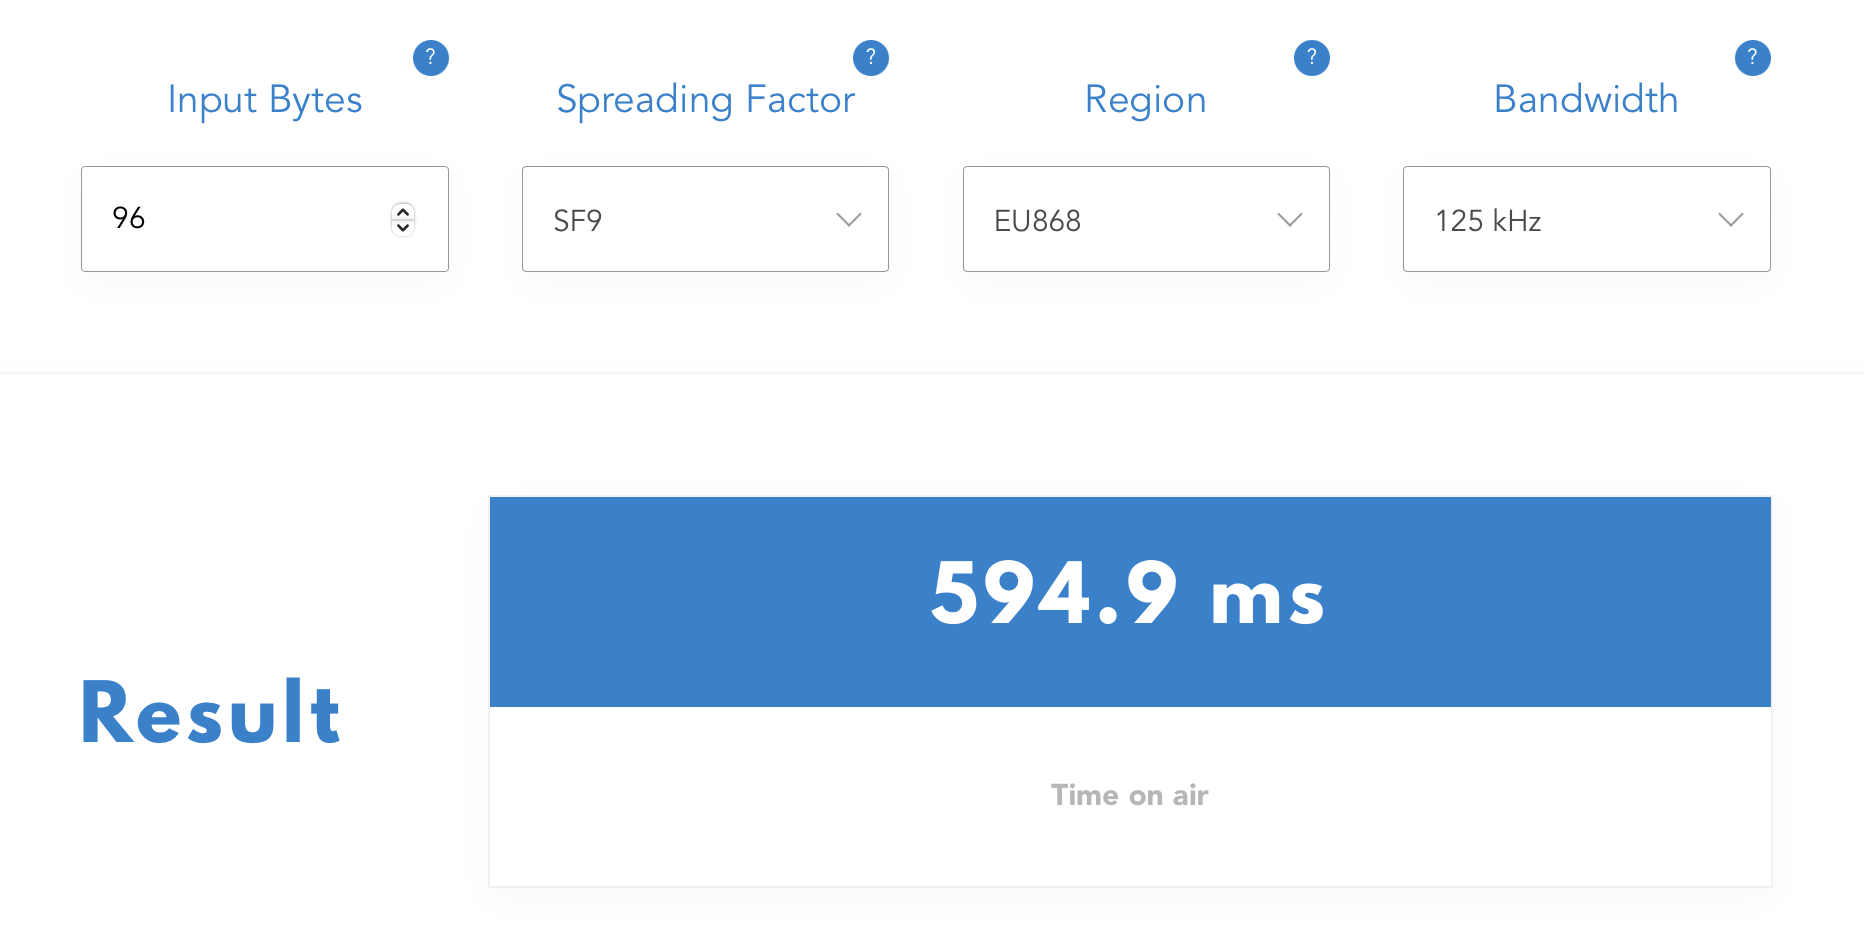
\includegraphics[width=0.6\linewidth, height=0.5\textheight, keepaspectratio]{sf9.png}
    \caption{Airtime with SF9}
\end{figure}

\begin{figure}[H]
    \centering
    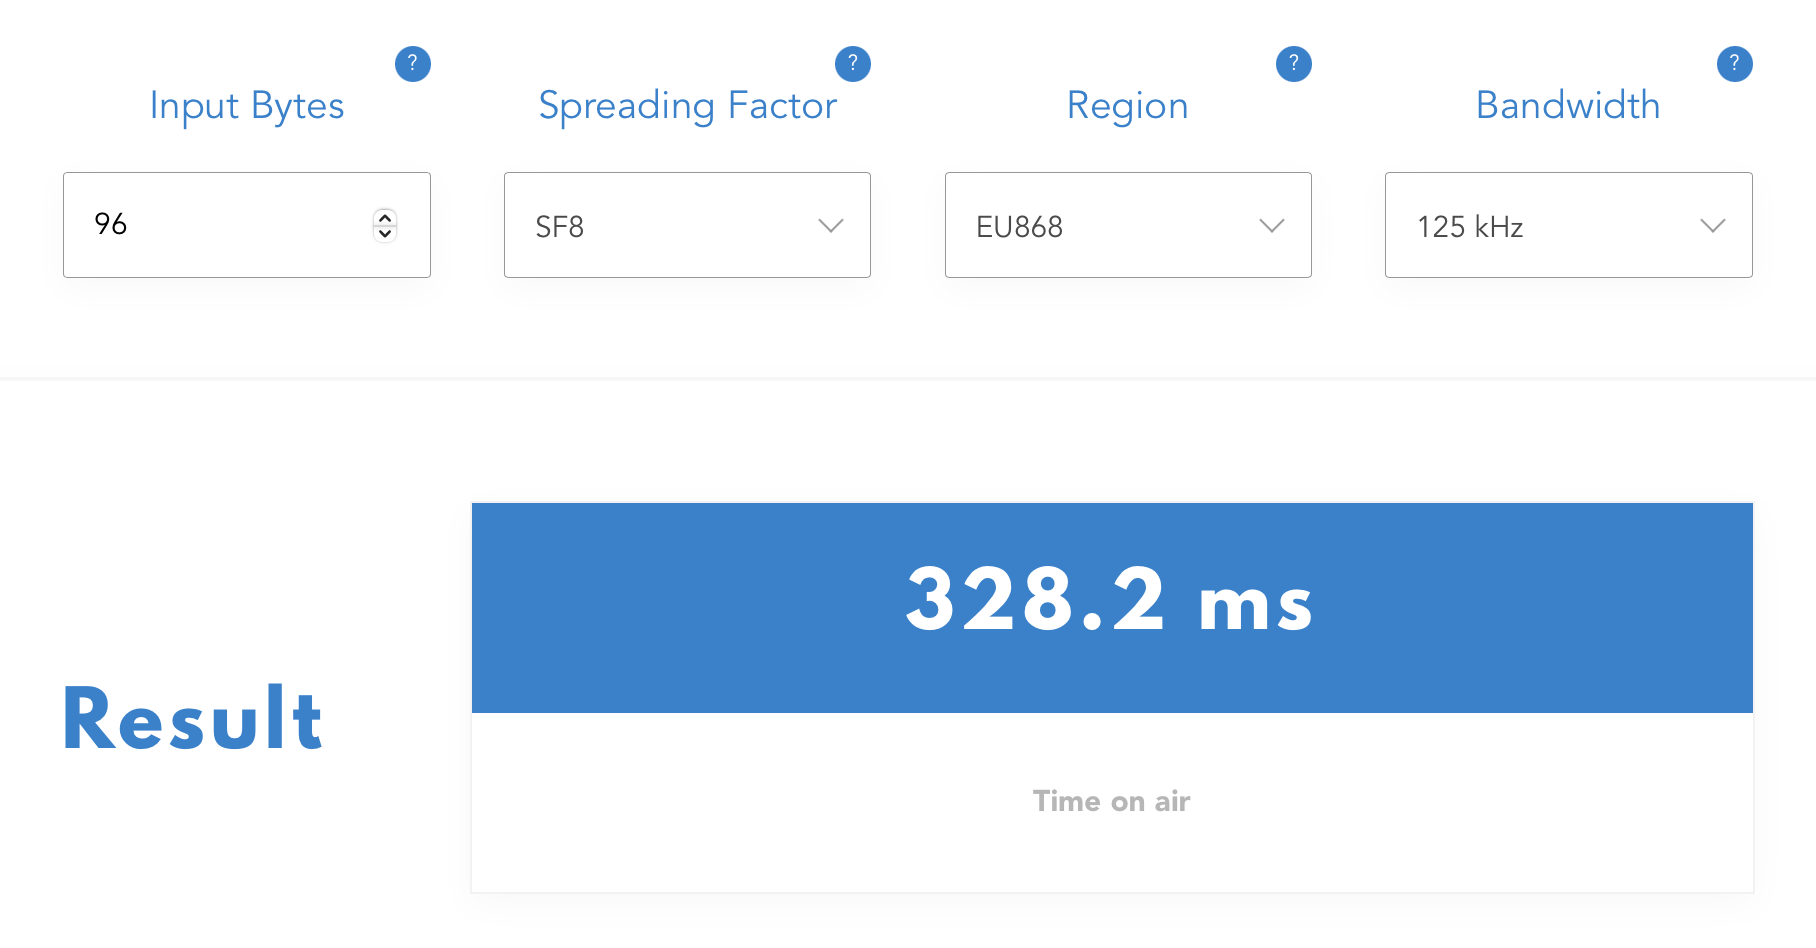
\includegraphics[width=0.6\linewidth, height=0.5\textheight, keepaspectratio]{sf8.png}
    \caption{Airtime with SF8}
\end{figure}

\begin{figure}[H]
    \centering
    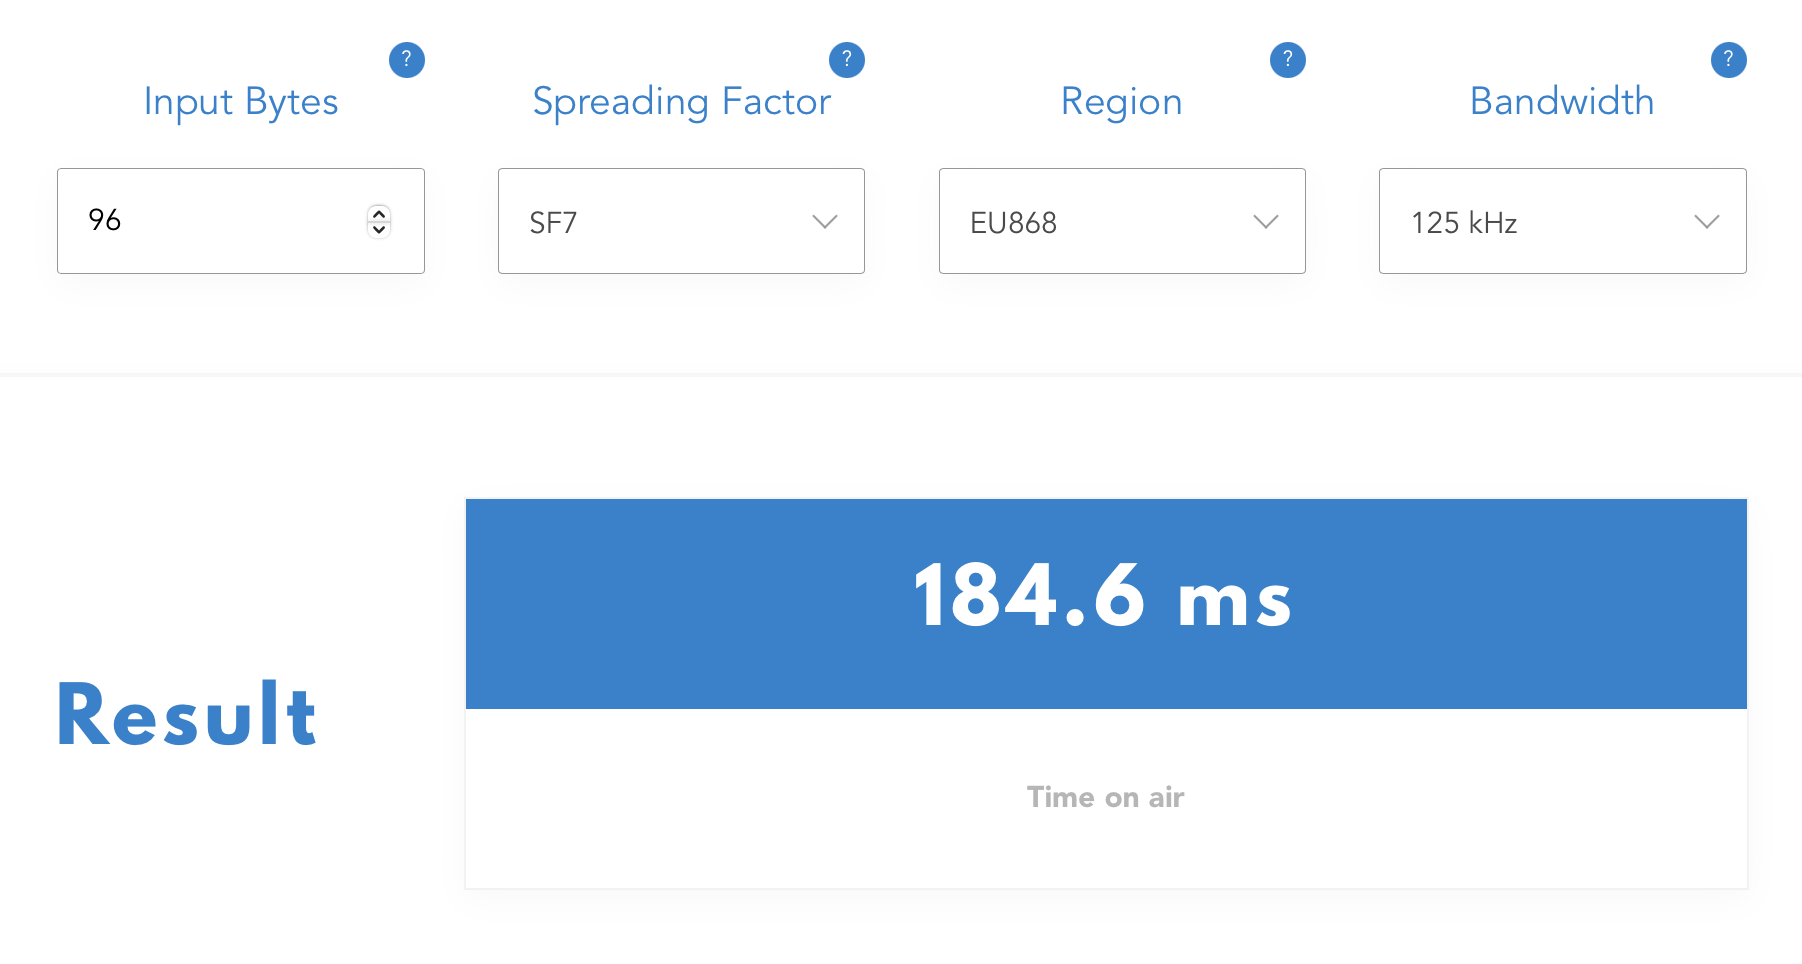
\includegraphics[width=0.6\linewidth, height=0.5\textheight, keepaspectratio]{sf7.png}
    \caption{Airtime with SF7}
\end{figure}






\chapter{EQ3 - Use LoRaSim to replicate simulations}
\label{ch:chapter_one}%
In this chapter we use the paper "Do LoRa Low-Power Wide-Area Networks Scale?" by M. Bor et al. and the LoRa simulator LoRaSim to reproduce the figures reporting the results of two Experiments Sets from the paper. LoRaSim is a simulator based on SimPy for simulating collisions in LoRa networks and consists in four Python scripts simulating different types of network, that can be run setting some parameters. In order to replicate the two figures, we need to understand which transmitter configuration was user for every configuration SN\textsuperscript{i} and use the correct simulator with the correct parameters.

\section{Figure 5: Experiment Set 2}
The Experiment Set 2 evaluates the impact of dynamic communication parameter selection on the Data Extraction Rate (DER) and compares three transmitter configurations, called  SN\textsuperscript{3}, SN\textsuperscript{4} and SN\textsuperscript{5} in the paper.\\
First of all, we need to choose the correct Python script in the simulator; the paper says that nodes transmit to a single sink (M=1), so we choose the script loraDir.py. From the LoRaSim documentation, we check the parameters used from the selected script, that are reported here:
\begin{BreakableVerbatim}
./loraDir.py <NODES> <AVGSEND> <EXPERIMENT> <SIMTIME> [COLLISION]
\end{BreakableVerbatim}
For all experiments, we choose:
\begin{itemize}
\item The number of nodes, <NODES>, is chosen from a list built based on the data point of Figure 5 from the paper.
\item The average sending interval in milliseconds, <AVGSEND>, is set to 1 million of milliseconds, i.e. 16.7 minutes.
\item The simulation time, <SIMTIME>, is not specified from the paper; we choose a simulation time of 58 days, the same as the one used in Experiment Set 1.
\item We set <COLLISION> to 1 to enable the full collision check.
\end{itemize}
The key difference between the different configurations is represented by the <EXPERIMENT> parameter that determines with which radio settings the simulation is run. We are going to choose the experiment looking at how the Experiment Set is described and at the LoRaSim documentation. The paper says that SN\textsuperscript{3} uses the settings used by common LoRaWAN deployments, which refers to <EXPERIMENT> = 4. SN\textsuperscript{4}, instead, is the configuration that minimizes the airtime for each node, by setting the BW, SF and CR, with constant TP; this description corresponds to <EXPERIMENT> = 3. Finally, SN\textsuperscript{5} minimizes first airtime and then Transmission Power, as done by the simulator with <EXPERIMENT> = 5.

The complete code used to simulate the network with LoRaSim and plot the DER is reported here.
\begin{python}
import os
import subprocess
import math
import pandas as pd
import matplotlib
import matplotlib.pyplot as plt

def simulate(n_nodes, tx_rate, exp, duration):
    env = os.environ.copy()
    env["MPLBACKEND"] = "Agg"
    # Use subprocess.run to execute the command and capture output
    result = subprocess.run(
        [
            "python2",
            "lorasim/loraDir.py",
            str(int(n_nodes)),
            str(int(tx_rate)),
            str(int(exp)),
            str(int(duration)),
            str(int(1))
        ],
        env=env,
        capture_output=True,
        text=True,  # Capture output as text
    )

# Der in aloha defined as S/G = e^(-2G)
def aloha_der(n_nodes,t):
    rate = 1e-6
    return math.exp(-2 * n_nodes * rate * t)

def main():
    duration = 58 * 86400000
    tx_rate = 1e6

    for n_nodes in list(range(1,10)) + list(range(10,100,10)) + list(range(100,1000,100)) + list(range(1000,1601,200)):
        print(f"Simulating {n_nodes} nodes")
        simulate(n_nodes, tx_rate, 4, duration)
        simulate(n_nodes, tx_rate, 3, duration)
        simulate(n_nodes, tx_rate, 5, duration)

    data_sn3 = pd.read_csv("exp4.dat", sep=" ")
    data_sn4 = pd.read_csv("exp3.dat", sep=" ")
    data_sn5 = pd.read_csv("exp5.dat", sep=" ")
    data_sn3["der"] = (data_sn3["nrTransmissions"] - data_sn3["nrCollisions"]) / data_sn3["nrTransmissions"]
    data_sn4["der"] = (data_sn4["nrTransmissions"] - data_sn4["nrCollisions"]) / data_sn4["nrTransmissions"]
    data_sn5["der"] = (data_sn5["nrTransmissions"] - data_sn5["nrCollisions"]) / data_sn5["nrTransmissions"]
    
    plt.plot(data_sn3["#nrNodes"], data_sn3["der"], marker = 'o', label="SN3")
    plt.plot(data_sn4["#nrNodes"], data_sn4["der"], marker = 'o', label="SN4")
    plt.plot(data_sn5["#nrNodes"], data_sn5["der"], marker = 'o', label="SN5")
    plt.title("Success Rate (%)")
    plt.xlabel("Number of nodes")
    plt.ylabel("Rate")
    plt.legend()
    plt.grid()

    plt.savefig("figure5.pdf")
    plt.show()

if __name__ == '__main__':
    main()
\end{python}

The plot that corresponds to Figure 5 from the paper is reported here.

\begin{figure}[H]
    \centering
    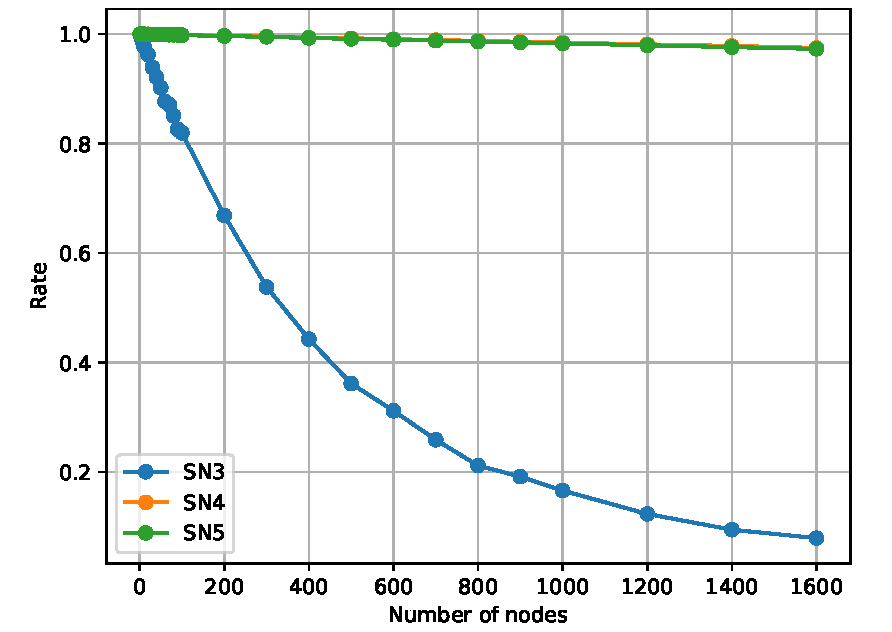
\includegraphics[width=0.7\linewidth, height=0.5\textheight, keepaspectratio]{figure5_58d_collision.pdf}
    \caption{Plot corresponding to Figure 5: Experiment Set 2}
\end{figure}

\section{Figure 7: Experiment Set 3}
The Experiment Set 3 analyzes the impact of the number of sinks M on the network performance, while Figure 7 focuses on the impact on the DER. The experiment uses the configuration called SN\textsuperscript{1}, with SF = 12, BW = 125 kHz and CR = 4/8, and tests different numbers of sinks (1, 2, 3, 4, 8, 24).\\
The Python script of the LoRaSim simulator that allows to test multiple sinks is loraDirMulBs.py and takes the following parameters:
\begin{BreakableVerbatim}
./loraDirMulBS.py <NODES> <AVGSEND> <EXPERIMENT> <SIMTIME> <BASESTATIONS> [COLLISION]
\end{BreakableVerbatim}
The only new parameter with respect to the previous Experiment Set is <BASESTATIONS> which is the number of gateways we have in the network. 
The parameters that are common to Experiment Set 2 are: 
\begin{itemize}
\item Parameter <NODES>, chosen from the same list of numbers.
\item <AVGSEND> is set to 1 million of milliseconds.
\item <COLLISION> is set to 1.
\end{itemize}
We modified the <SIMTIME> to 1 day, because it is not specified by the paper and Google Colab can't handle a very long simulation time for this Experiment Set, since it saturates the available RAM. The paper says that the used setting is the one of SN\textsuperscript{1}, which uses the most robust LoRa transmitter settings leading to transmissions with the longest possible airtime and with fixed Carrier Frequency. This description refers to <EXPERIMENT> = 0, which uses a constant frequency. The number of gateways, contained in the parameter <BASESTATIONS> changes among the different simulations and is set to 1, 2, 3, 4, 8 and 24, as done in the paper.
The complete code used to simulate the network with LoRaSim and plot the DER is reported here.

\begin{python}
import os
import subprocess
import math
import pandas as pd
import matplotlib
import matplotlib.pyplot as plt

def simulate(n_nodes, tx_rate, exp, duration):
    env = os.environ.copy()
    env["MPLBACKEND"] = "Agg"

    # Use subprocess.run to execute the command and capture output
    result = subprocess.run(
        [
            "python2",
            "lorasim/loraDir.py",
            str(int(n_nodes)),
            str(int(tx_rate)),
            str(int(exp)),
            str(int(duration)),
            str(int(1))
        ],
        env=env,
        capture_output=True,
        text=True,  # Capture output as text
    )

# Der in aloha defined as S/G = e^(-2G)
def aloha_der(n_nodes,t):
    rate = 1e-6
    return math.exp(-2 * n_nodes * rate * t)

def main():
    duration = 30 * 86400000
    tx_rate = 1e6

    for n_nodes in list(range(1,10)) + list(range(10,100,10)) + list(range(100,1000,100)) + list(range(1000,1601,200)):
        print(f"Simulating {n_nodes} nodes")
        simulate(n_nodes, tx_rate, 0, duration, 1)
        simulate(n_nodes, tx_rate, 0, duration, 2)
        simulate(n_nodes, tx_rate, 0, duration, 3)
        simulate(n_nodes, tx_rate, 0, duration, 4)
        simulate(n_nodes, tx_rate, 0, duration, 8)
        simulate(n_nodes, tx_rate, 0, duration, 24)

    data_bs_1 = pd.read_csv("exp0BS1.dat", delim_whitespace=True, comment="#", names=["nrNodes", "DER"])
    data_bs_2 = pd.read_csv("exp0BS2.dat", delim_whitespace=True, comment="#", names=["nrNodes", "DER"])
    data_bs_3 = pd.read_csv("exp0BS3.dat",delim_whitespace=True, comment="#", names=["nrNodes", "DER"])
    data_bs_4 = pd.read_csv("exp0BS4.dat", delim_whitespace=True, comment="#", names=["nrNodes", "DER"])
    data_bs_8 = pd.read_csv("exp0BS8.dat", delim_whitespace=True, comment="#", names=["nrNodes", "DER"])
    data_bs_24 = pd.read_csv("exp0BS24.dat", delim_whitespace=True, comment="#", names=["nrNodes", "DER"])
   
    plt.plot(data_bs_1["nrNodes"], data_bs_1["DER"], marker = 'o', label="1 sink")
    plt.plot(data_bs_2["nrNodes"], data_bs_2["DER"], marker = 'o', label="2 sink")
    plt.plot(data_bs_3["nrNodes"], data_bs_3["DER"], marker = 'o', label="3 sink")
    plt.plot(data_bs_4["nrNodes"], data_bs_4["DER"], marker = 'o', label="4 sink")
    plt.plot(data_bs_8["nrNodes"], data_bs_8["DER"], marker = 'o', label="8 sink")
    plt.plot(data_bs_24["nrNodes"], data_bs_24["DER"], marker = 'o', label="24 sink")
    plt.title("Success Rate (%)")
    plt.xlabel("Number of nodes")
    plt.ylabel("Rate")
    plt.legend()
    plt.grid()
    plt.savefig("figure7.pdf")
    plt.show()

if __name__ == '__main__':
    main()

\end{python}

The plot that corresponds to Figure 7 from the paper is reported here.
\begin{figure}[H]
    \centering
    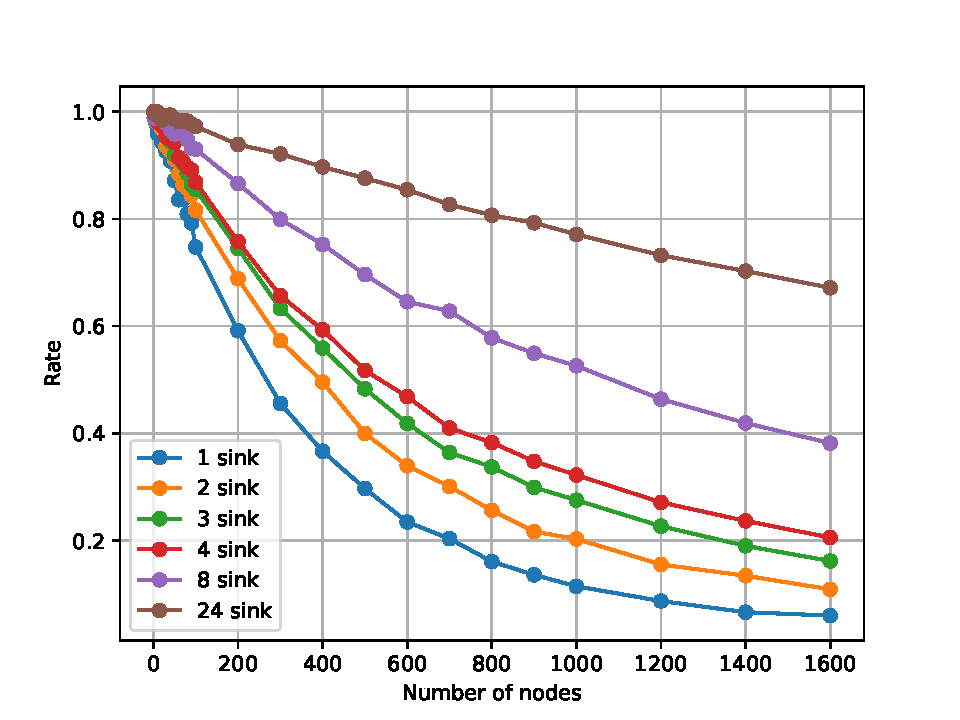
\includegraphics[width=0.7\linewidth, height=0.5\textheight, keepaspectratio]{figure7_exp0_1d_collision.pdf}
    \caption{Plot corresponding to Figure 7: Experiment Set 3}
\end{figure}





%-------------------------------------------------------------------------
%	BIBLIOGRAPHY
%-------------------------------------------------------------------------

\addtocontents{toc}{\vspace{2em}} % Add a gap in the Contents, for aesthetics
\bibliography{Thesis_bibliography} % The references information are stored in the file named "Thesis_bibliography.bib"

%-------------------------------------------------------------------------
%	APPENDICES
%-------------------------------------------------------------------------

% LIST OF FIGURES
\listoffigures

% LIST OF TABLES
\listoftables


\end{document}

